\documentclass[11pt, letterpaper]{memoir}
\usepackage{HomeworkStyle}

\begin{document}
	\begin{center}
		{\large	Quiz 11.1 -- The Solvation Process}
	\end{center}
	{\large Name: \rule[-1mm]{4in}{.1pt} 

	\subsection*{Question 1}
  For each common solution, list the \emph{solvent} and the \emph{solute} or \emph{solutes}
  \begin{itemize}
    \item The air around us

      ~
    \item Steel

      ~
    \item Tears

      ~
    \item Everclear ($\geq120$ proof liquor)

      ~
  \end{itemize}

	\subsection*{Question 2}
  For each type of attractive force listed below, indicate whether they are \emph{broken} or \emph{formed} in the solvation process

  \noindent{\large Solvent-Solvent \hspace{5em} Solvent-Solute \hspace{5em} Solute-Solute}

  \vspace{2em}
  \subsection*{Question 3}
  Refer to the figure of solubilities below. For each condition listed, indicate whether the solution is \emph{saturated}, \emph{unsaturated}, or \emph{supersaturated}

  \noindent
  \begin{minipage}{0.4\linewidth}
    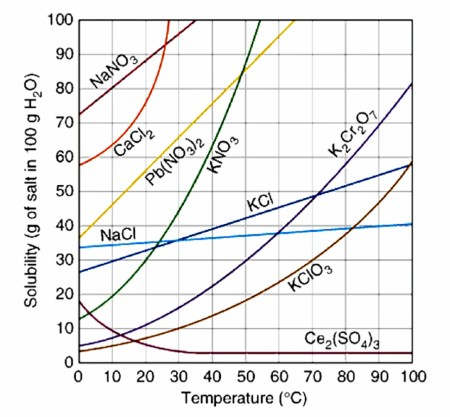
\includegraphics[width=\linewidth]{Solubilities}
  \end{minipage}
  \begin{minipage}{0.6\linewidth}
    \begin{itemize}
      \item $50g$ \ch{KCl} in $120g$ \ch{H2O} at $70^\circ C$ 

        ~
      \item $12g$ \ch{Pb(NO3)2} in $75g$ \ch{H2O} at $20^\circ C$ 

        ~
      \item $80g$ \ch{NaNO3} in $100g$ \ch{H2O} at $10^\circ C$ 

        ~
      \item $10g$ \ch{Ce2(SO4)3} in $150g$ \ch{H2O} at $5^\circ C$ 

        ~
      \item $10g$ \ch{Ce2(SO4)3} in $150g$ \ch{H2O} at $85^\circ C$ 
    \end{itemize}
  \end{minipage}
	\newpage
	\pagestyle{empty}
	\addtocounter{page}{-1}
  \newgeometry{hmargin=0.85in,vmargin=0.85in}
  \section*{\emph{For Whom the Bell Tolls}}
  \paragraph{By John Donne}~

  \begin{verse}
  No man is an island,\\
  Entire of itself.\\
  Each is a piece of the continent,\\
  A part of the main.\\
  If a clod be washed away by the sea,\\
  Europe is the less.\\
  As well as if a promontory were.\\
  As well as if a manor of thine own\\
  Or of thine friend's were.\\
  Each man's death diminishes me,\\
  For I am involved in mankind.\\
  Therefore, send not to know\\
  For whom the bell tolls,\\
  It tolls for thee.\\
  \end{verse}

  \hspace{18em}
  \begin{minipage}{0.7\linewidth}
    \section*{\emph{Streets}}
    \paragraph{By Naomi Shihab Nye}

    \begin{verse}
    A man leaves the world\\
    and the streets he lived on\\
    grow a little shorter.

    One more window dark\\
    in this city, the figs on his branches\\
    will soften for birds.

    If we stand quietly enough evenings\\
    there grows a whole company of us\\
    standing quietly together.\\
    overhead loud grackles are claiming their trees  \\
    and the sky which sews and sews, tirelessly sewing,\\
    drops her purple hem.\\
    Each thing in its time, in its place,\\
    it would be nice to think the same about people.

    Some people do. They sleep completely,\\
    waking refreshed. Others live in two worlds,\\
    the lost and remembered.\\
    They sleep twice, once for the one who is gone,\\
    once for themselves. They dream thickly,\\
    dream double, they wake from a dream\\
    into another one, they walk the short streets\\
    calling out names, and then they answer.
    \end{verse}
  \end{minipage}
\end{document}
